\section{Convolutional Neural Networks}
\subsection{Introduction}
\emph{Convolutional Neural Networks} (CNNs) is a class of models widely used in computer vision. While Fully Connected Neural Networks are very powerful machine learning models, they do not respect the 2D spatial structure of the input images. For instance, training a Multilayer Perceptron on a dataset of $32\times 32$ images required the model to start with a \texttt{Flatten} layer, that reshaped matrix images of size \texttt{(32, 32)} to flattened vectors of size \texttt{(1024, 1)}. Similarly, different color channels were handled separately, reshaping tensor images of dimensions \texttt{(32, 32, 3)} to \texttt{(3072, 1)}.

\begin{figure}[H]
    \centering
    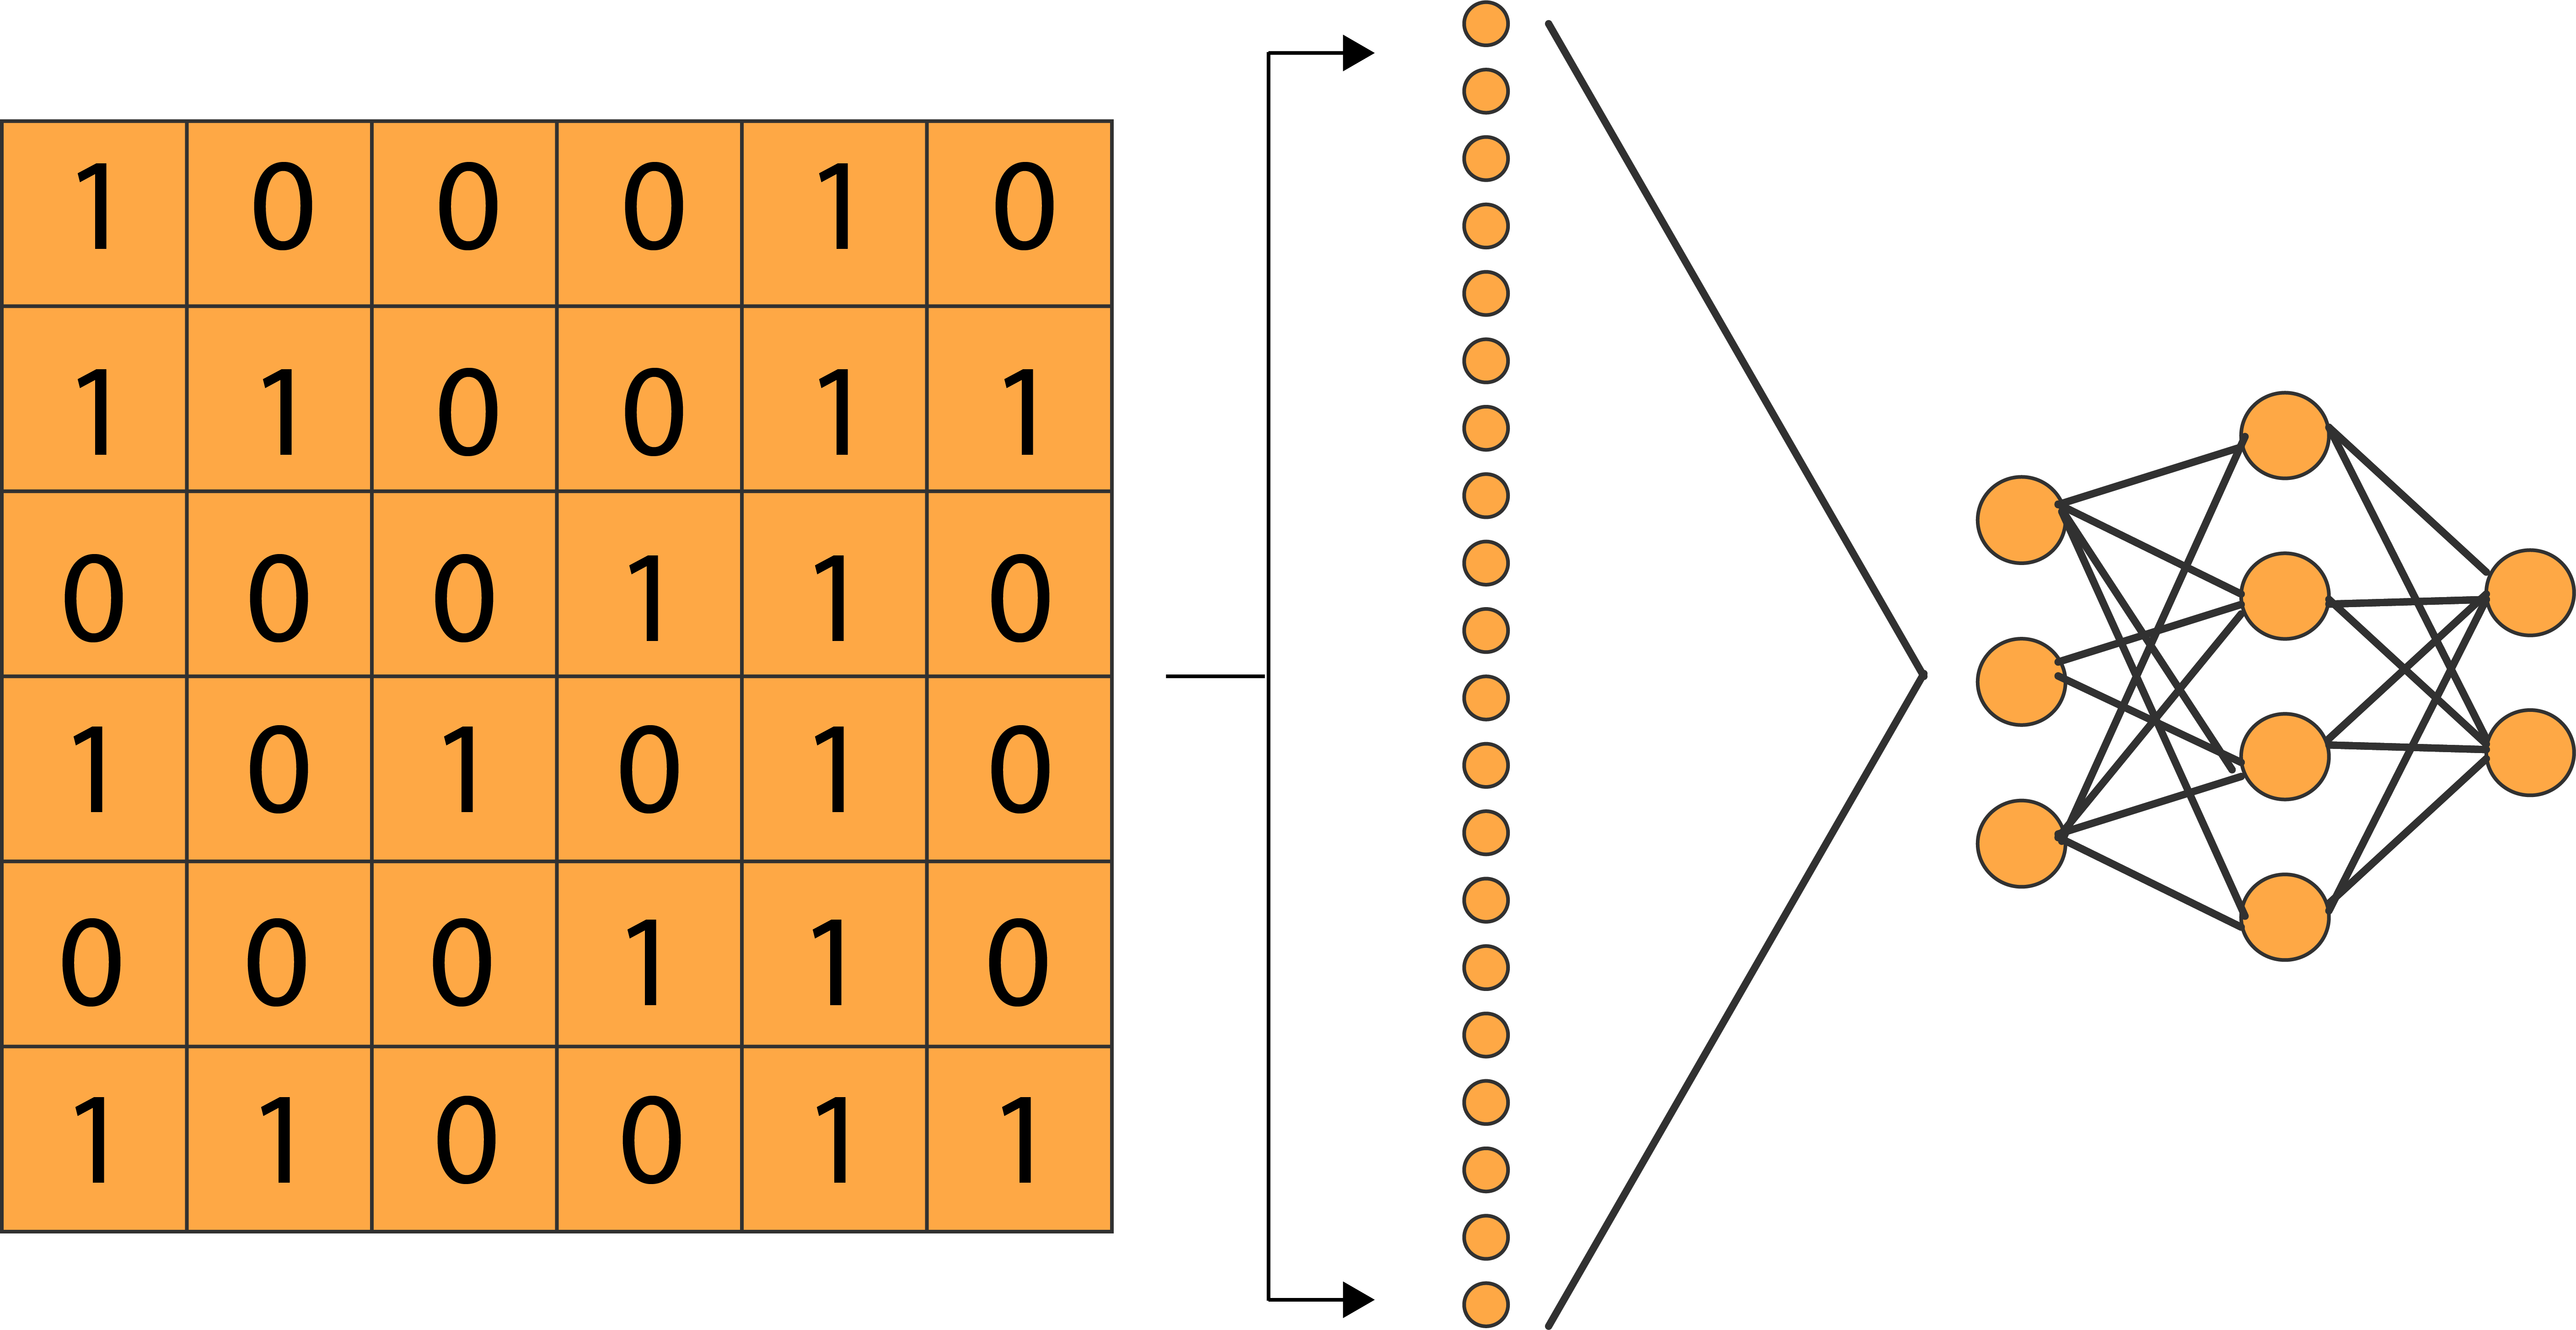
\includegraphics[width=0.5\textwidth]{images/flatten.png}
    \caption{Flatten layer breaking the spatial strucutre of input data}
\end{figure}

CNNs introduce new operators taking advantage of the spatial structure of the input data, while remaining compatible with automatic differentiation. While MLPs build the basic blocks of Deep Neural Networks using Fully-Connected Layers and Activation Layers, this chapter will introduce three new types of layers: \emph{Convolution Layers}, \emph{Pooling Layers}, and \emph{Normalization}.

\subsection{Convolution Layers}
Similarly to Fully-Connected Layers, \emph{Convolution Layers} have learnable weights, but also have the particularity to respect the spatial information.

\subsubsection{Input shape}
A Fully-Connected layer receives some flattened vector and outputs another vector:
\begin{figure}[H]
    \centering
    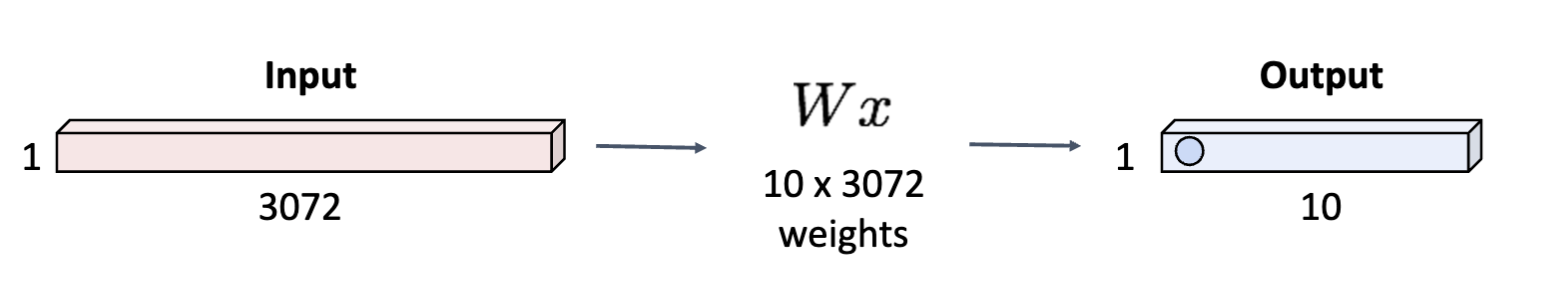
\includegraphics[width=0.8\textwidth]{images/fully-connected.png}
    \caption{Fully-Connected Layer}
\end{figure}

Instead, a CNN takes as an input a 3D volume: for instance, an image can be represented as a tensor of shape $3\times32\times32$, the first dimension being the number of channels (red, green, blue), and the other two being the width and height of the image.

\subsubsection{Kernels}
The convolutional layer itself consists of small kernels (also called filters) used to \emph{convolve} with the image, that is sliding over it spatially, and computing the dot products at each possible location.
\begin{definition}[Kernel]
    A \emph{kernel} (or \emph{filter}) is a tensor of dimensions $D\times K\times K$, where $D$ is the number of channels (or \say{depth}) of the input, and $K$ is a parameter called \emph{kernel size}.
\end{definition}

\begin{definition}[Convolution of two matrices]
    Given two matrices $A=(a_{i, j})_{i, j}$ and $B=(b_{i, j})_{i, j}$ in $\mathscr{M}_{m, n}(\R)$, the \emph{convolution of $A$ and $B$}, noted $A*B\in\R$, is the following:
    \begin{equation}
        A*B = \sum_{i=1}^m \sum_{j=1}^n a_{(m-i+1), (n-j+1)} \cdot b_{i, j}
    \end{equation}
    This corresponds to the dot product in the space $\mathscr{M}_{m, n}(\R)$.
\end{definition}

\begin{definition}[Kernel convolution]
    An input of shape $D\times H\times W$ can be processed by a kernel of shape $D\times K\times K$ by computing at each possible spatial position the convolution between the kernel and the submatrix of the input. 
    \begin{figure}[H]
        \centering
        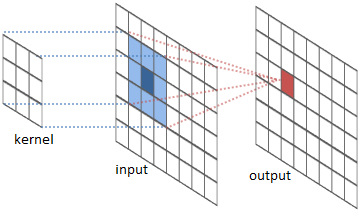
\includegraphics[width=0.4\textwidth]{images/convolution-simple.png}
        \caption{Kernel convolution}
    \end{figure}
    
    The output of this operation in an \emph{activation map} of dimension $1\times (H - K + 1) \times (W - K + 1)$ representing for each pixel the convolution between the kernel and corresponding chunk of the image.
    \begin{figure}[H]
        \centering
        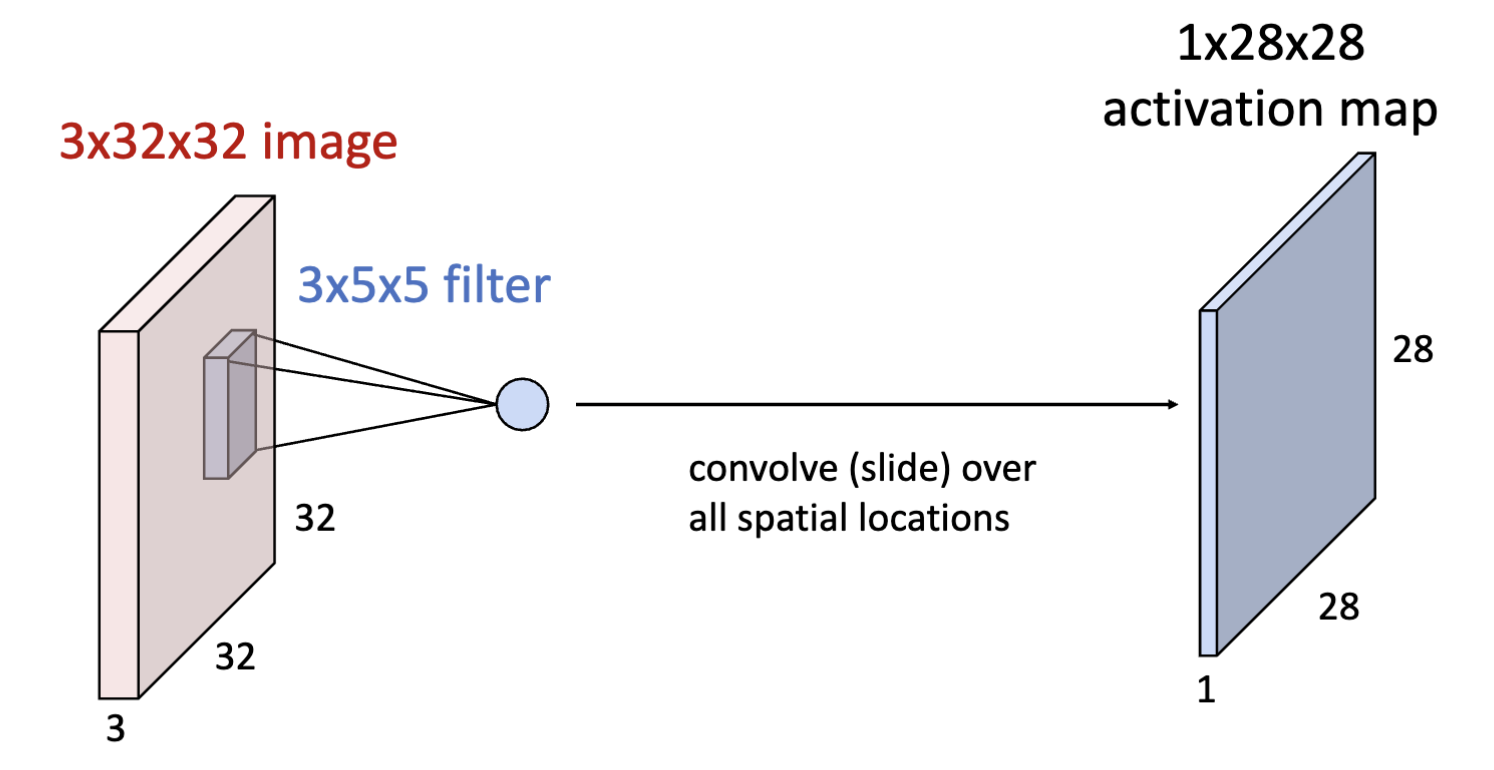
\includegraphics[width=0.6\textwidth]{images/convolutional-map.png}
        \caption{Input and output of the convolution operation}
        \label{fig:one-kernel-layer}
    \end{figure}
\end{definition}

Intuitively, the result of the kernel convolution tells us for each pixel \emph{how much the neighbourhood of the input pixel corresponds to the kernel}.

\begin{example}[Gaussian blur]
    Let $G\in\mathscr{M}_{3}(\R)$ be the following kernel:
    \begin{equation*}
        G := \frac{1}{16}\begin{bmatrix}
            1 & 2 & 1\\
            2 & 4 & 1\\
            1 & 2 & 1
        \end{bmatrix}
    \end{equation*}
    Each coefficient of this matrix is an approximation of the Gaussian distribution. Applying this kernel to an image produces a smoothed version of the input.
\end{example}
% TODO: add gaussian blur image

\begin{example}[Sobel operator]
    Let $S_x$ and $S_y\in\mathscr{M}_{3}(\R)$ be the following kernels:
    \begin{equation*}
        S_x := \begin{bmatrix}
            +1 & 0 & -1\\
            +2 & 0 & -2\\
            +1 & 0 & -1
        \end{bmatrix}
        \qquad\textnormal{and}\qquad
        S_y := S_x^\tp = \begin{bmatrix}
            +1 & +2 & +1\\
            \phantom{+}0 & \phantom{+}0 & \phantom{+}0\\
            -1 & -2 & -1
        \end{bmatrix}
    \end{equation*}
    The convolution between these operators and an image produces horizontal and vertical derivatives approximations of the image pixels.

    \begin{figure}[H]
        \centering
    
        \begin{minipage}{0.4\textwidth}
            \centering
            \caption*{Input image}
            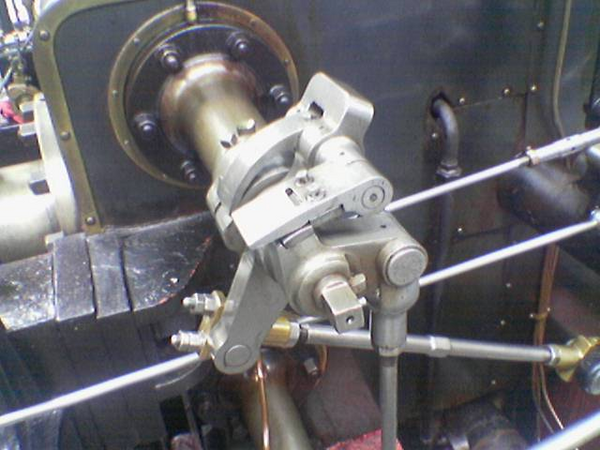
\includegraphics[width=.7\textwidth]{images/pre-sobel.png}
        \end{minipage}
        \begin{minipage}{0.4\textwidth}
            \centering
            \caption*{Sobel operator applied to the image}
            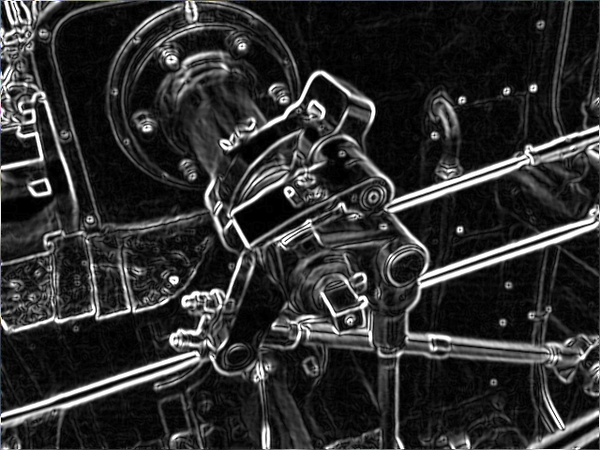
\includegraphics[width=.7\textwidth]{images/post-sobel.png}
        \end{minipage}
        
        \caption{Effect of the Sobel operator on an image}
    \end{figure}
\end{example}

These two examples show that kernels used in convolutional layers express meaningful transformations of the input, justifying their use in CNNs. For instance, one could hardcode different kernels (gaussian blur, Sobel operator, vertical/horizontal lines extraction) to extract interesting features from an image, and plug these features into an MLP to obtain an improved classifier compared to a basic, flattening MLP. We will see that instead, CNNs have learnable kernel weights, allowing the model to choose the kernels that it considers bests.

\subsubsection{Multiple kernels}
In Figure \ref{fig:one-kernel-layer}, we used simply one kernel to compute one activation map. In practice, we repeat this process multiple times: we consider a set (or \emph{bank}) of filters having different weights values, and for each kernel of the set, we compute its activation map.
\begin{figure}[H]
    \centering
    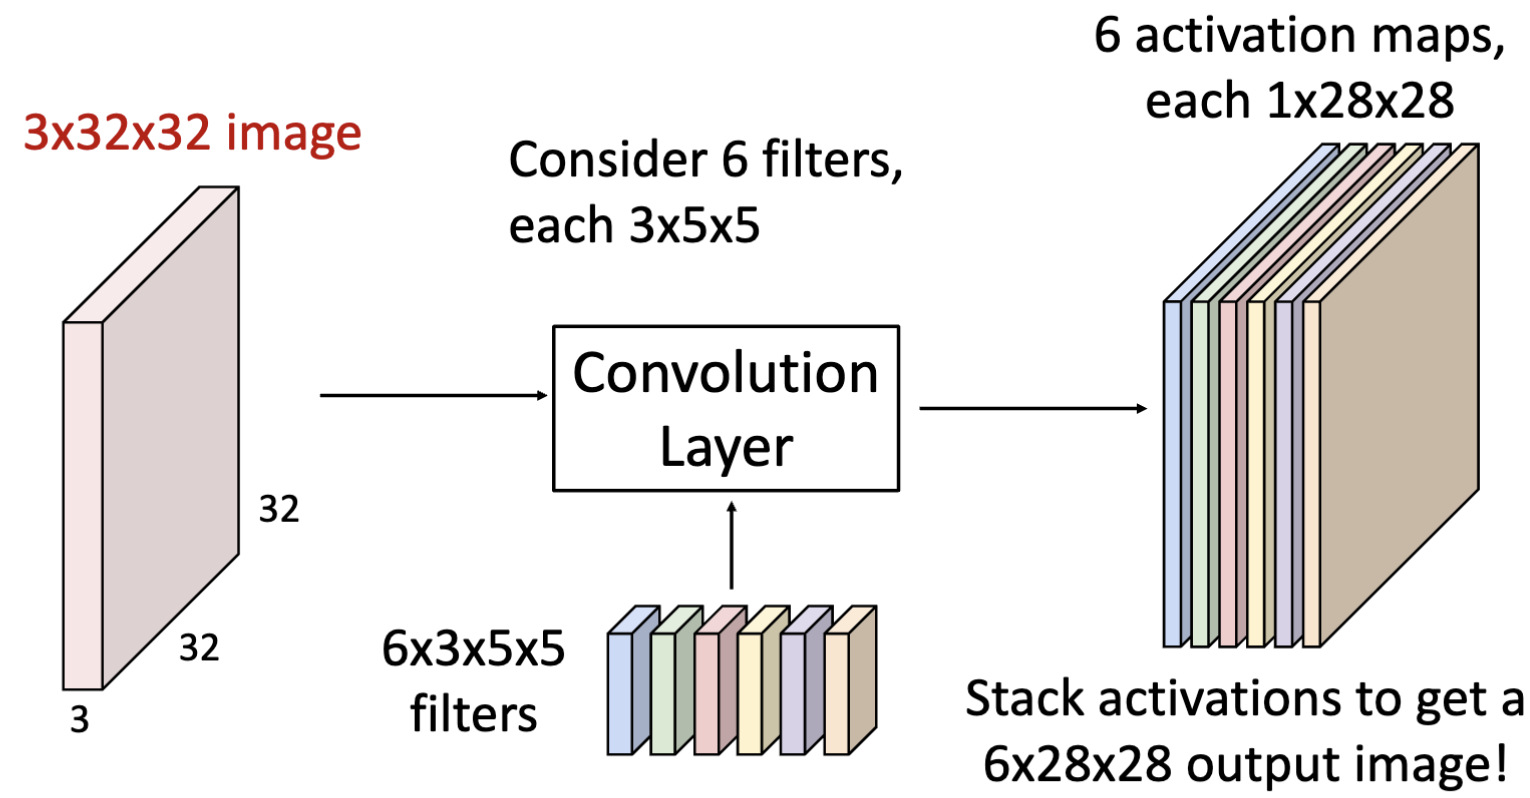
\includegraphics[width=0.6\textwidth]{images/multiple-kernels.png}
    \caption{Convolutional Layer using 6 kernels}
\end{figure}